\documentclass[]{tufte-handout}

% ams
\usepackage{amssymb,amsmath}

\usepackage{ifxetex,ifluatex}
\usepackage{fixltx2e} % provides \textsubscript
\ifnum 0\ifxetex 1\fi\ifluatex 1\fi=0 % if pdftex
  \usepackage[T1]{fontenc}
  \usepackage[utf8]{inputenc}
\else % if luatex or xelatex
  \makeatletter
  \@ifpackageloaded{fontspec}{}{\usepackage{fontspec}}
  \makeatother
  \defaultfontfeatures{Ligatures=TeX,Scale=MatchLowercase}
  \makeatletter
  \@ifpackageloaded{soul}{
     \renewcommand\allcapsspacing[1]{{\addfontfeature{LetterSpace=15}#1}}
     \renewcommand\smallcapsspacing[1]{{\addfontfeature{LetterSpace=10}#1}}
   }{}
  \makeatother
\fi

% graphix
\usepackage{graphicx}
\setkeys{Gin}{width=\linewidth,totalheight=\textheight,keepaspectratio}

% booktabs
\usepackage{booktabs}

% url
\usepackage{url}

% hyperref
\usepackage{hyperref}

% units.
\usepackage{units}


\setcounter{secnumdepth}{-1}

% citations

% pandoc syntax highlighting
\usepackage{color}
\usepackage{fancyvrb}
\newcommand{\VerbBar}{|}
\newcommand{\VERB}{\Verb[commandchars=\\\{\}]}
\DefineVerbatimEnvironment{Highlighting}{Verbatim}{commandchars=\\\{\}}
% Add ',fontsize=\small' for more characters per line
\newenvironment{Shaded}{}{}
\newcommand{\KeywordTok}[1]{\textbf{{#1}}}
\newcommand{\DataTypeTok}[1]{\underline{{#1}}}
\newcommand{\DecValTok}[1]{{#1}}
\newcommand{\BaseNTok}[1]{{#1}}
\newcommand{\FloatTok}[1]{{#1}}
\newcommand{\ConstantTok}[1]{{#1}}
\newcommand{\CharTok}[1]{{#1}}
\newcommand{\SpecialCharTok}[1]{{#1}}
\newcommand{\StringTok}[1]{{#1}}
\newcommand{\VerbatimStringTok}[1]{{#1}}
\newcommand{\SpecialStringTok}[1]{{#1}}
\newcommand{\ImportTok}[1]{{#1}}
\newcommand{\CommentTok}[1]{\textit{{#1}}}
\newcommand{\DocumentationTok}[1]{\textit{{#1}}}
\newcommand{\AnnotationTok}[1]{\textit{{#1}}}
\newcommand{\CommentVarTok}[1]{\textit{{#1}}}
\newcommand{\OtherTok}[1]{{#1}}
\newcommand{\FunctionTok}[1]{{#1}}
\newcommand{\VariableTok}[1]{{#1}}
\newcommand{\ControlFlowTok}[1]{\textbf{{#1}}}
\newcommand{\OperatorTok}[1]{{#1}}
\newcommand{\BuiltInTok}[1]{{#1}}
\newcommand{\ExtensionTok}[1]{{#1}}
\newcommand{\PreprocessorTok}[1]{\textbf{{#1}}}
\newcommand{\AttributeTok}[1]{{#1}}
\newcommand{\RegionMarkerTok}[1]{{#1}}
\newcommand{\InformationTok}[1]{\textit{{#1}}}
\newcommand{\WarningTok}[1]{\textit{{#1}}}
\newcommand{\AlertTok}[1]{\textbf{{#1}}}
\newcommand{\ErrorTok}[1]{\textbf{{#1}}}
\newcommand{\NormalTok}[1]{{#1}}

% longtable
\usepackage{longtable,booktabs}

% multiplecol
\usepackage{multicol}

% strikeout
\usepackage[normalem]{ulem}

% morefloats
\usepackage{morefloats}


% tightlist macro required by pandoc >= 1.14
\providecommand{\tightlist}{%
  \setlength{\itemsep}{0pt}\setlength{\parskip}{0pt}}

% title / author / date
\title{Journals Included in Literature Search}
\author{Riley M. Smith}
\date{22 March 2017}

\bibliographystyle{tufte}
% \usepackage{caption}
\usepackage{cleveref}
%
% --------------------- %
% Latex Logo Commands
% --------------------- %
%
\usepackage{xspace}
\newcommand{\latex}{\LaTeX\xspace}
\newcommand{\tex}{\TeX\xspace}
\newcommand{\bibtex}{\textsc{Bib}\tex}
%
% --------------------- %
% Colors
% --------------------- %
%
\usepackage{color}
\definecolor{magenta}{rgb}{0.79, 0.08, 0.48} %% ~c9147a %%
\definecolor{dkmagenta}{rgb}{0.55, 0.0, 0.55} %% ~8c008c %%
\definecolor{dpmagenta}{rgb}{0.8, 0.0, 0.8} %% ~140014 %%
\definecolor{patriarch}{rgb}{0.5, 0.0, 0.5} %% ~0d000d %%
\definecolor{dkpatriarch}{rgb}{0.4, 0.0, 0.4} %% ~0a000a %%
\definecolor{blue}{rgb}{0.07, 0.04, 0.56} %% ~120a8f %%
\definecolor{royalblue}{rgb}{0.0, 0.22, 0.66} %% ~0038a8 %%
\definecolor{dkblue}{rgb}{0.0, 0.0, 0.55} %% ~00008c %%
\definecolor{mnblue}{rgb}{0.1, 0.1, 0.44} %% ~030370 %%
\definecolor{smblue}{rgb}{0.0, 0.2, 0.6} %% ~00050f %%
\definecolor{Rblue}{rgb}{0.39, 0.35, 0.639} %% ~0a09a3 %%
\definecolor{dkmnblue}{rgb}{0.0, 0.2, 0.4} %% ~00050a %%
\definecolor{navy}{rgb}{0.0, 0.0, 0.5} %% ~00000d %%
\definecolor{dknavy}{rgb}{0, 0, .208} %% ~000035 %%
\definecolor{blublk}{rgb}{0, 0, .106} %% ~00001b %%
\definecolor{blugray}{rgb}{0.33, 0.41, 0.47} %% ~546978 %%
\definecolor{grayblue}{rgb}{0.33, 0.41, 0.58} %% ~~546994 %%
\definecolor{slgray}{rgb}{0.44, 0.5, 0.56} %% ~70808d %%
\definecolor{red}{rgb}{.545, 0.0, 0.0} %% ~8b0000 %%
\definecolor{dkred}{rgb}{.247, 0.0, 0.0} %% ~3f0000 %%
\definecolor{mplblu}{HTML}{363283}
%
\definecolor{pdxgray}{HTML}{373737} %% ~373737 %%
\definecolor{pdxgreen}{HTML}{8B9535} %% ~8B9535 %%
\definecolor{myblack}{HTML}{181C20} %% ~181C20 %%
%
% ---------------------------------------- %
% Indent first line of text in tabular env %
% ---------------------------------------- %
%
\newcommand{\rowgroup}[2][-1em]{\hspace{#1}#2}
\newcommand{\mrowgroup}[3]{\hspace*{#1}#2\hspace*{#1}#3}
%
% --------------------- %
% Format Block Quotes
% --------------------- %
%   Size: Scriptsize
%   Reduce vertical space above
%   Color: Gray
%
\usepackage{setspace}
% \expandafter\def\expandafter\quote\expandafter{\quote\small\singlespacing\color{myblack!65}\vspace{-0.5\baselineskip}}

% \expandafter\def\expandafter\quote\expandafter{\quote\small\singlespacing\vspace{-1em}}

% \setlength\listindent{1em}

\usepackage{enumitem}
\setlist[itemize, 1]{leftmargin=!, labelindent=0.5em, itemindent=-3em, label=\scriptsize{$\cdot$}, partopsep=0em, topsep=0.15em}
% \setlist[itemize, 2]{leftmargin=4em, label=$\centerdot$, topsep=0em}
% \setlength{\itemindent}{5in}

%
% ------------------- %
% Make Links Standout
% ------------------- %
%   (E.Tufte does not believe in using colors in links. I disagree.) %
%
% \newcommand{\rurl}[1]{\underline{\color{dkblue}{\url{~1}}}}
% \newcommand{\rhref}[2]{\underline{\color{dkblue}{\href{~1}{~2}}}}
\hypersetup{breaklinks=true,colorlinks=true,linkcolor=navy,urlcolor=navy}
%
% ------------------- %
% Format "texttt"
% ------------------- %
%
\newcommand{\rtt}[1]{\color{patriarch}{\texttt{#1}}}
%
\usepackage{amsmath}
%
% ----------------------------- %
% Command to insert "ToDo" tags
% ----------------------------- %
%
\newcommand{\todo}{\textbf{\color{red}{\texttt{[ToDo]}}}}
\newcommand{\inprogress}{\textbf{\textit{\color{blue}{\texttt{[In Progress]}}}}}
\newcommand{\complete}{\sout{\textit{\color{slgray}{\texttt{[Complete]}}}}}

\usepackage{enumitem,amssymb}
\newlist{todolist}{itemize}{2}
\setlist[todolist]{label=$\square$}
\newcommand{\todoitem}[1]{\textit{\color{red}{#1}}}

\newcommand{\textbft}[1]{\underline{\textbf{\texttt{#1}}}}


% ---------------------------%
% Code Formatting %
% ---------------------------%
% \usepackage{highlight}

% \definecolor{fgcolor}{rgb}{0.196, 0.196, 0.196}
% \newcommand{\hlnum}[1]{\textcolor[rgb]{0.063,0.58,0.627}{#1}}%
% \newcommand{\hlstr}[1]{\textcolor[rgb]{0.063,0.58,0.627}{#1}}%
% \newcommand{\hlcom}[1]{\textcolor[rgb]{0.588,0.588,0.588}{#1}}%
% \newcommand{\hlopt}[1]{\textcolor[rgb]{0.196,0.196,0.196}{#1}}%
% \newcommand{\hlstd}[1]{\textcolor[rgb]{0.196,0.196,0.196}{#1}}%
% \newcommand{\hlkwa}[1]{\textcolor[rgb]{0.231,0.416,0.784}{#1}}%
% \newcommand{\hlkwb}[1]{\textcolor[rgb]{0.627,0,0.314}{#1}}%
% \newcommand{\hlkwc}[1]{\textcolor[rgb]{0,0.631,0.314}{#1}}%
% \newcommand{\hlkwd}[1]{\textcolor[rgb]{0.78,0.227,0.412}{#1}}%

\let\hlipl\hlkwb
% \newcommand{\Rrule}{\textcolor{Rblue}{\rule{\linewidth}{0.05mm}}\newline
\includegraphics[width=0.5cm]{auxDocs/Rlogo.png}}
\usepackage{dashrule}

\newcommand{\Rrule}{
    % \setlength{\parindent}{-10pt}
    \vspace*{1em}
    \noindent
    \hspace{-1em}
    
\includegraphics[width=0.5cm]{auxDocs/Rlogo.png}
    \textcolor{Rblue}{
        \rule[0.1in]{0.90\linewidth}{0.02mm}
    }
    \vspace{-1.35em}
}

\newcommand{\Rerule}{
    % \setlength{\parindent}{-0.5in}
    \noindent
    \hspace{-1em}
    \textcolor{Rblue}{
        $\llcorner$\rule[-0.4mm]{\linewidth}{0.02mm}
                % \hfill
                % $\lrcorner$
    }
}

\newcommand{\Rruleb}{
    % \setlength{\parindent}{-10pt}
    \vspace*{1em}
    \noindent
    \hspace{-1em}
    
\includegraphics[width=0.5cm]{auxDocs/Rlogo-bw.png}
    \textcolor{slgray}{
        \rule[0.1in]{0.90\textwidth}{0.02mm}
    }
    \vspace{-1.35em}
}

\newcommand{\Reruleb}{
    % \setlength{\parindent}{-0.5in}
    \noindent
    \hspace{-1em}
    \textcolor{slgray}{
        $\llcorner$\rule[-0.4mm]{\textwidth}{0.02mm}
                % \hfill
                % $\lrcorner$
    }
}

\newcommand{\MPrule}{
    % \setlength{\parindent}{-10pt}
    \vspace*{1em}
    \noindent
    \hspace{-1em}
    
\includegraphics[width=0.5cm]{../auxDocs/mplus.png}
    \textcolor{mplblu}{
        \rule[0.1in]{0.90\textwidth}{0.02mm}
    }
    \vspace{-1.5em}
}

\newcommand{\MPerule}{
    % \setlength{\parindent}{-0.5in}
    \noindent
    \hspace{-1em}
    \textcolor{mplblu}{
        $\llcorner$\rule[-0.4mm]{\textwidth}{0.02mm}
                % \hfill
                % $\lrcorner$
    }
}

\newcommand{\Frule}{
    \vspace*{-1em}
    \begin{fullwidth}\textcolor{blublk}{\rule{\linewidth}{0.2mm}}\end{fullwidth}
}

% \newcommand{\Rrule}{
%     \noindent
%     \textcolor{Rblue}{
%         $\ulcorner\textregistered$\hdashrule[0.015in]{
%             0.9\linewidth
%             }
%             {1pt}{1pt}
%         $\textregistered\urcorner$
%         }}
% \newcommand{\Rerule}{
%     \noindent
%     \textcolor{Rblue}{
%         $\llcorner\textregistered$\hdashrule[0.025in]{
%             0.9\linewidth
%             }
%             {1pt}{1pt}
%         $\textregistered\lrcorner$
%         }}
% \newcommand{\Rerule}{\noindent\textcolor{Rblue}{\vdash\hdashrule[-0.015in]{\linewidth}{1pt}{1pt}\dashv}

% \vdash - \dashv
% \perp
% \ll - \gg
% +
% \pm
% \mp
% \ \newcommand{\Rrule}{\noindent
\includegraphics[width=0.5cm]{auxDocs/Rlogo.png}\textcolor{Rblue}{\hdashrule[0.25in]{\linewidth}{1pt}{1pt}}}
% \newcommand{\Rrule}{\noindent
\includegraphics[width=0.5cm]{auxDocs/Rlogo.png}\textcolor{Rblue}{\rule[0.25in]{\linewidth}{0.05mm}}}

% \newcommand{\Rerule}{\textcolor{Rblue}{\rule{\linewidth}{0.05mm}}}
% \hdashrule [⟨raise⟩] [⟨leader⟩] {⟨width⟩} {⟨height⟩} {⟨dash⟩}

%%%%%%%%%%%%%%%%%%%%%%%%%%
% Wrapper for Chi-Square %
%%%%%%%%%%%%%%%%%%%%%%%%%%

\newcommand{\chisq}{\chi^{2}}
\newcommand{\sq}{^{2}}

\newcommand{\tdef}[3][-0.5em]{\tufteskip\noindent\rowgroup[#1]{\textsc{#2}} \newline {#3}}
\newcommand{\hf}{\hfill}
\DeclareMathAlphabet{\mathpzc}{OT1}{pzc}{m}{it} %% to make \mathpzc typeset its argument in Zapf Chancery (see page 16 of "The Great, Big List of LATEX Symbols" by David Carlisle, Scott Pakin, & Alexander Holt (2001)) %%

\newcommand{\df}{\mathpzc{df}}

\begin{document}

\maketitle




\Frule

\section[Community Psychology Journals]{\texorpdfstring{Community
Psychology Journals\footnote{\url{http://www.scra27.org/publications/other-journals-relevant-community-psychology/}}}{Community Psychology Journals}}\label{community-psychology-journals}

\Rrule

\begin{Shaded}
\begin{Highlighting}[]
\NormalTok{JOURNAL <-}\StringTok{ }\KeywordTok{c}\NormalTok{(}\StringTok{"Action Research"}\NormalTok{,}
             \StringTok{"American Journal of Community Psychology"}\NormalTok{,}
             \StringTok{"American Journal of Health Promotion"}\NormalTok{,}
             \StringTok{"American Journal of Orthopsychiatry"}\NormalTok{,}
             \StringTok{"American Journal of Preventive Medicine"}\NormalTok{,}
             \StringTok{"American Journal of Public Health"}\NormalTok{,}
             \StringTok{"Australian Community Psychologist"}\NormalTok{,}
             \StringTok{"Community Development"}\NormalTok{,}
             \StringTok{"Community Development Journal"}\NormalTok{,}
             \StringTok{"Community Mental Health Journal"}\NormalTok{,}
             \StringTok{"Community Psychology in Global Perspective"}\NormalTok{,}
             \StringTok{"Cultural Diversity and Ethnic Minority Psychology"}\NormalTok{,}
             \StringTok{"Global Journal of Community Psychology Practice"}\NormalTok{,}
             \StringTok{"Health Education and Behavior"}\NormalTok{,}
             \StringTok{"Health Promotion Practice"}\NormalTok{,}
             \StringTok{"Journal of Applied Social Psychology"}\NormalTok{,}
             \StringTok{"Journal of Community and Applied Social Psychology"}\NormalTok{,}
             \StringTok{"Journal of Community Practice"}\NormalTok{,}
             \StringTok{"Journal of Health and Social Behavior"}\NormalTok{,}
             \StringTok{"Journal of Prevention and Intervention"}\NormalTok{,}
             \StringTok{"Journal of Primary Prevention"}\NormalTok{,}
             \StringTok{"Journal of Rural Community Psychology"}\NormalTok{,}
             \StringTok{"Journal of Social Issues"}\NormalTok{,}
             \StringTok{"Journal of Community Psychology"}\NormalTok{,}
             \StringTok{"Psychiatric Rehabilitation Journal"}\NormalTok{,}
             \StringTok{"Psychology of Women Quarterly"}\NormalTok{,}
             \StringTok{"Psychosocial Intervention"}\NormalTok{,}
             \StringTok{"Social Science and Medicine"}\NormalTok{,}
             \StringTok{"The Community Psychologist"}\NormalTok{,}
             \StringTok{"Transcultural Psychiatry"}\NormalTok{,}
             \StringTok{"Progress in Community Health Partnerships: Research, Education, and Action"}\NormalTok{)}
\end{Highlighting}
\end{Shaded}

\begin{Shaded}
\begin{Highlighting}[]
\NormalTok{Year <-}\StringTok{ }\KeywordTok{c}\NormalTok{(}\DecValTok{2003}\NormalTok{, }\DecValTok{1973}\NormalTok{, }\DecValTok{1986}\NormalTok{, }\DecValTok{1930}\NormalTok{, }\DecValTok{1985}\NormalTok{, }\DecValTok{1971}\NormalTok{, }\DecValTok{2006}\NormalTok{, }\DecValTok{2005}\NormalTok{, }\DecValTok{1966}\NormalTok{, }\DecValTok{1965}\NormalTok{, }\DecValTok{2015}\NormalTok{, }
    \DecValTok{1995}\NormalTok{, }\DecValTok{2010}\NormalTok{, }\DecValTok{1997}\NormalTok{, }\DecValTok{2000}\NormalTok{, }\DecValTok{1971}\NormalTok{, }\DecValTok{1991}\NormalTok{, }\DecValTok{1994}\NormalTok{, }\DecValTok{1967}\NormalTok{, }\DecValTok{1996}\NormalTok{, }\DecValTok{1981}\NormalTok{, }\DecValTok{1980}\NormalTok{, }\DecValTok{1997}\NormalTok{, }
    \DecValTok{1973}\NormalTok{, }\DecValTok{1996}\NormalTok{, }\DecValTok{1976}\NormalTok{, }\DecValTok{2011}\NormalTok{, }\DecValTok{1967}\NormalTok{, }\DecValTok{1975}\NormalTok{, }\DecValTok{1997}\NormalTok{, }\DecValTok{2007}\NormalTok{)}

\NormalTok{SJR <-}\StringTok{ }\KeywordTok{c}\NormalTok{(}\FloatTok{0.33}\NormalTok{, }\FloatTok{1.237}\NormalTok{, }\FloatTok{0.821}\NormalTok{, }\FloatTok{0.756}\NormalTok{, }\FloatTok{2.764}\NormalTok{, }\FloatTok{2.52}\NormalTok{, }\OtherTok{NA}\NormalTok{, }\OtherTok{NA}\NormalTok{, }\FloatTok{0.47}\NormalTok{, }\FloatTok{0.467}\NormalTok{, }\OtherTok{NA}\NormalTok{, }
    \OtherTok{NA}\NormalTok{, }\OtherTok{NA}\NormalTok{, }\FloatTok{1.177}\NormalTok{, }\FloatTok{0.769}\NormalTok{, }\FloatTok{0.639}\NormalTok{, }\FloatTok{0.855}\NormalTok{, }\FloatTok{0.278}\NormalTok{, }\FloatTok{1.727}\NormalTok{, }\FloatTok{0.231}\NormalTok{, }\FloatTok{0.64}\NormalTok{, }\OtherTok{NA}\NormalTok{, }
    \FloatTok{1.467}\NormalTok{, }\FloatTok{0.425}\NormalTok{, }\FloatTok{0.692}\NormalTok{, }\FloatTok{1.216}\NormalTok{, }\FloatTok{0.331}\NormalTok{, }\FloatTok{1.894}\NormalTok{, }\OtherTok{NA}\NormalTok{, }\FloatTok{1.141}\NormalTok{, }\FloatTok{0.427}\NormalTok{)}

\NormalTok{H <-}\StringTok{ }\KeywordTok{c}\NormalTok{(}\DecValTok{15}\NormalTok{, }\DecValTok{83}\NormalTok{, }\DecValTok{72}\NormalTok{, }\DecValTok{69}\NormalTok{, }\DecValTok{154}\NormalTok{, }\DecValTok{196}\NormalTok{, }\OtherTok{NA}\NormalTok{, }\OtherTok{NA}\NormalTok{, }\DecValTok{28}\NormalTok{, }\DecValTok{51}\NormalTok{, }\OtherTok{NA}\NormalTok{, }\OtherTok{NA}\NormalTok{, }\OtherTok{NA}\NormalTok{, }\DecValTok{72}\NormalTok{, }\DecValTok{32}\NormalTok{, }\DecValTok{78}\NormalTok{, }
    \DecValTok{44}\NormalTok{, }\DecValTok{15}\NormalTok{, }\DecValTok{93}\NormalTok{, }\DecValTok{21}\NormalTok{, }\DecValTok{36}\NormalTok{, }\OtherTok{NA}\NormalTok{, }\DecValTok{89}\NormalTok{, }\DecValTok{65}\NormalTok{, }\DecValTok{48}\NormalTok{, }\DecValTok{66}\NormalTok{, }\DecValTok{8}\NormalTok{, }\DecValTok{177}\NormalTok{, }\OtherTok{NA}\NormalTok{, }\DecValTok{35}\NormalTok{, }\DecValTok{15}\NormalTok{)}

\NormalTok{Med <-}\StringTok{ }\KeywordTok{c}\NormalTok{(}\DecValTok{0}\NormalTok{, }\DecValTok{1}\NormalTok{, }\DecValTok{1}\NormalTok{, }\DecValTok{1}\NormalTok{, }\DecValTok{1}\NormalTok{, }\DecValTok{1}\NormalTok{, }\DecValTok{0}\NormalTok{, }\DecValTok{0}\NormalTok{, }\DecValTok{0}\NormalTok{, }\DecValTok{1}\NormalTok{, }\DecValTok{0}\NormalTok{, }\DecValTok{0}\NormalTok{, }\DecValTok{1}\NormalTok{, }\DecValTok{1}\NormalTok{, }\DecValTok{1}\NormalTok{, }\DecValTok{0}\NormalTok{, }\DecValTok{0}\NormalTok{, }\DecValTok{0}\NormalTok{, }\DecValTok{1}\NormalTok{, }\DecValTok{1}\NormalTok{, }\DecValTok{1}\NormalTok{, }
    \DecValTok{1}\NormalTok{, }\DecValTok{0}\NormalTok{, }\DecValTok{0}\NormalTok{, }\DecValTok{1}\NormalTok{, }\DecValTok{0}\NormalTok{, }\DecValTok{0}\NormalTok{, }\DecValTok{1}\NormalTok{, }\DecValTok{1}\NormalTok{, }\DecValTok{1}\NormalTok{, }\DecValTok{0}\NormalTok{)}

\NormalTok{Psych <-}\StringTok{ }\KeywordTok{c}\NormalTok{(}\DecValTok{0}\NormalTok{, }\DecValTok{1}\NormalTok{, }\DecValTok{0}\NormalTok{, }\DecValTok{1}\NormalTok{, }\DecValTok{0}\NormalTok{, }\DecValTok{0}\NormalTok{, }\DecValTok{1}\NormalTok{, }\DecValTok{0}\NormalTok{, }\DecValTok{0}\NormalTok{, }\DecValTok{0}\NormalTok{, }\DecValTok{1}\NormalTok{, }\DecValTok{1}\NormalTok{, }\DecValTok{1}\NormalTok{, }\DecValTok{0}\NormalTok{, }\DecValTok{0}\NormalTok{, }\DecValTok{1}\NormalTok{, }\DecValTok{1}\NormalTok{, }\DecValTok{0}\NormalTok{, }\DecValTok{1}\NormalTok{, }\DecValTok{1}\NormalTok{, }
    \DecValTok{0}\NormalTok{, }\DecValTok{1}\NormalTok{, }\DecValTok{0}\NormalTok{, }\DecValTok{1}\NormalTok{, }\DecValTok{0}\NormalTok{, }\DecValTok{1}\NormalTok{, }\DecValTok{1}\NormalTok{, }\DecValTok{0}\NormalTok{, }\DecValTok{1}\NormalTok{, }\DecValTok{0}\NormalTok{, }\DecValTok{0}\NormalTok{)}

\NormalTok{SocSci <-}\StringTok{ }\KeywordTok{c}\NormalTok{(}\DecValTok{1}\NormalTok{, }\DecValTok{1}\NormalTok{, }\DecValTok{1}\NormalTok{, }\DecValTok{0}\NormalTok{, }\DecValTok{0}\NormalTok{, }\DecValTok{0}\NormalTok{, }\DecValTok{1}\NormalTok{, }\DecValTok{1}\NormalTok{, }\DecValTok{1}\NormalTok{, }\DecValTok{1}\NormalTok{, }\DecValTok{1}\NormalTok{, }\DecValTok{1}\NormalTok{, }\DecValTok{1}\NormalTok{, }\DecValTok{0}\NormalTok{, }\DecValTok{0}\NormalTok{, }\DecValTok{0}\NormalTok{, }\DecValTok{1}\NormalTok{, }\DecValTok{1}\NormalTok{, }\DecValTok{0}\NormalTok{, }\DecValTok{0}\NormalTok{, }
    \DecValTok{0}\NormalTok{, }\DecValTok{1}\NormalTok{, }\DecValTok{1}\NormalTok{, }\DecValTok{1}\NormalTok{, }\DecValTok{0}\NormalTok{, }\DecValTok{1}\NormalTok{, }\DecValTok{0}\NormalTok{, }\DecValTok{1}\NormalTok{, }\DecValTok{1}\NormalTok{, }\DecValTok{1}\NormalTok{, }\DecValTok{1}\NormalTok{)}

\NormalTok{Biz <-}\StringTok{ }\KeywordTok{c}\NormalTok{(}\DecValTok{1}\NormalTok{, }\KeywordTok{rep}\NormalTok{(}\DecValTok{0}\NormalTok{, }\DecValTok{30}\NormalTok{))}

\NormalTok{AH <-}\StringTok{ }\KeywordTok{c}\NormalTok{(}\DecValTok{0}\NormalTok{, }\DecValTok{0}\NormalTok{, }\DecValTok{0}\NormalTok{, }\DecValTok{1}\NormalTok{, }\DecValTok{0}\NormalTok{, }\DecValTok{0}\NormalTok{, }\DecValTok{0}\NormalTok{, }\DecValTok{0}\NormalTok{, }\DecValTok{0}\NormalTok{, }\DecValTok{0}\NormalTok{, }\DecValTok{0}\NormalTok{, }\DecValTok{0}\NormalTok{, }\DecValTok{0}\NormalTok{, }\DecValTok{1}\NormalTok{, }\DecValTok{0}\NormalTok{, }\DecValTok{0}\NormalTok{, }\DecValTok{0}\NormalTok{, }\DecValTok{0}\NormalTok{, }\DecValTok{0}\NormalTok{, }\DecValTok{0}\NormalTok{, }\DecValTok{0}\NormalTok{, }
    \DecValTok{0}\NormalTok{, }\DecValTok{0}\NormalTok{, }\DecValTok{0}\NormalTok{, }\DecValTok{0}\NormalTok{, }\DecValTok{1}\NormalTok{, }\DecValTok{0}\NormalTok{, }\DecValTok{1}\NormalTok{, }\DecValTok{0}\NormalTok{, }\DecValTok{0}\NormalTok{, }\DecValTok{0}\NormalTok{)}

\NormalTok{Nurs <-}\StringTok{ }\KeywordTok{c}\NormalTok{(}\KeywordTok{rep}\NormalTok{(}\DecValTok{0}\NormalTok{, }\DecValTok{14}\NormalTok{), }\DecValTok{1}\NormalTok{, }\KeywordTok{rep}\NormalTok{(}\DecValTok{0}\NormalTok{, }\DecValTok{16}\NormalTok{))}

\NormalTok{HlthPrf <-}\StringTok{ }\KeywordTok{c}\NormalTok{(}\KeywordTok{rep}\NormalTok{(}\DecValTok{0}\NormalTok{, }\DecValTok{21}\NormalTok{), }\DecValTok{1}\NormalTok{, }\DecValTok{0}\NormalTok{, }\DecValTok{0}\NormalTok{, }\DecValTok{1}\NormalTok{, }\DecValTok{0}\NormalTok{, }\DecValTok{0}\NormalTok{, }\DecValTok{0}\NormalTok{, }\DecValTok{1}\NormalTok{, }\DecValTok{0}\NormalTok{, }\DecValTok{0}\NormalTok{)}

\NormalTok{Location <-}\StringTok{ }\KeywordTok{c}\NormalTok{(}\StringTok{"UK"}\NormalTok{, }\StringTok{"US"}\NormalTok{, }\StringTok{"US"}\NormalTok{, }\StringTok{"US"}\NormalTok{, }\StringTok{"US"}\NormalTok{, }\StringTok{"US"}\NormalTok{, }\StringTok{"AU"}\NormalTok{, }\StringTok{"UK"}\NormalTok{, }\StringTok{"UK"}\NormalTok{, }\StringTok{"NL"}\NormalTok{, }
    \StringTok{"IT"}\NormalTok{, }\StringTok{"US"}\NormalTok{, }\StringTok{"US"}\NormalTok{, }\StringTok{"US"}\NormalTok{, }\StringTok{"US"}\NormalTok{, }\StringTok{"UK"}\NormalTok{, }\StringTok{"UK"}\NormalTok{, }\StringTok{"US"}\NormalTok{, }\StringTok{"US"}\NormalTok{, }\StringTok{"US"}\NormalTok{, }\StringTok{"US"}\NormalTok{, }\StringTok{"US"}\NormalTok{, }
    \StringTok{"UK"}\NormalTok{, }\StringTok{"US"}\NormalTok{, }\StringTok{"US"}\NormalTok{, }\StringTok{"UK"}\NormalTok{, }\StringTok{"ES"}\NormalTok{, }\StringTok{"UK"}\NormalTok{, }\StringTok{"US"}\NormalTok{, }\StringTok{"UK"}\NormalTok{, }\StringTok{"US"}\NormalTok{)}

\NormalTok{dat <-}\StringTok{ }\KeywordTok{data.frame}\NormalTok{(JOURNAL, Location, Year, SJR, H)}

\NormalTok{dat.subj <-}\StringTok{ }\KeywordTok{data.frame}\NormalTok{(Med, Psych, SocSci, Biz, AH, Nurs, HlthPrf)}
\NormalTok{dat.subj$Nsubj <-}\StringTok{ }\KeywordTok{apply}\NormalTok{(dat.subj, }\DecValTok{1}\NormalTok{, sum)}
\NormalTok{dat <-}\StringTok{ }\KeywordTok{cbind}\NormalTok{(dat, dat.subj) %>%}\StringTok{ }\KeywordTok{as.data.frame}\NormalTok{()}
\NormalTok{dat.narm <-}\StringTok{ }\KeywordTok{na.omit}\NormalTok{(dat) %>%}\StringTok{ }\KeywordTok{as.data.frame}\NormalTok{()}
\KeywordTok{names}\NormalTok{(dat.narm) <-}\StringTok{ }\KeywordTok{c}\NormalTok{(}\StringTok{"Journal"}\NormalTok{, }\StringTok{"Location"}\NormalTok{, }\StringTok{"Year"}\NormalTok{, }\StringTok{"ScimagoJourn.Rating"}\NormalTok{, }
    \StringTok{"H-Index"}\NormalTok{, }\StringTok{"Medical"}\NormalTok{, }\StringTok{"Psychology"}\NormalTok{, }\StringTok{"SocialSciences"}\NormalTok{, }\StringTok{"Business"}\NormalTok{, }\StringTok{"Arts&Humanities"}\NormalTok{, }
    \StringTok{"Nursing"}\NormalTok{, }\StringTok{"HealthProfessions"}\NormalTok{, }\StringTok{"N_CoveredTopics"}\NormalTok{)}

\KeywordTok{cor}\NormalTok{(dat.narm[, -}\DecValTok{1}\NormalTok{:-}\DecValTok{2}\NormalTok{]) %>%}\StringTok{ }\NormalTok{corrplot::}\KeywordTok{corrplot.mixed}\NormalTok{(}\DataTypeTok{lower =} \StringTok{"number"}\NormalTok{, }\DataTypeTok{upper =} \StringTok{"shade"}\NormalTok{, }
    \DataTypeTok{tl.pos =} \StringTok{"lt"}\NormalTok{, }\DataTypeTok{diag =} \StringTok{"u"}\NormalTok{, }\DataTypeTok{bg =} \OtherTok{NA}\NormalTok{, }\DataTypeTok{col =} \KeywordTok{blgrmg}\NormalTok{(}\KeywordTok{length}\NormalTok{(}\KeywordTok{cor}\NormalTok{(dat.narm[, }
        \NormalTok{-}\DecValTok{1}\NormalTok{:-}\DecValTok{2}\NormalTok{]))), }\DataTypeTok{tl.col =} \NormalTok{mypal[}\DecValTok{19}\NormalTok{])}

\NormalTok{cl <-}\StringTok{ }\KeywordTok{mpal}\NormalTok{(H, }\DataTypeTok{p =} \NormalTok{cols3)}
\NormalTok{bg <-}\StringTok{ }\KeywordTok{adjustcolor}\NormalTok{(cl, }\DataTypeTok{alpha.f =} \FloatTok{0.6}\NormalTok{)}
\KeywordTok{with}\NormalTok{(dat, \{}
    \NormalTok{lm1 <-}\StringTok{ }\KeywordTok{lm}\NormalTok{(H ~}\StringTok{ }\NormalTok{SJR)}
    \KeywordTok{plot}\NormalTok{(SJR, H, }\DataTypeTok{col =} \NormalTok{cl, }\DataTypeTok{bg =} \NormalTok{bg, }\DataTypeTok{pch =} \DecValTok{21}\NormalTok{, }\DataTypeTok{xlab =} \StringTok{"Scimago Journal Rating"}\NormalTok{, }
        \DataTypeTok{ylab =} \StringTok{"H Index"}\NormalTok{)}
    \KeywordTok{abline}\NormalTok{(lm1, }\DataTypeTok{lwd =} \FloatTok{2.5}\NormalTok{, }\DataTypeTok{col =} \NormalTok{mypal[}\DecValTok{18}\NormalTok{])}
\NormalTok{\})}
\end{Highlighting}
\end{Shaded}

\includegraphics[width=\linewidth]{graphics/rplot-unnamed-chunk-2-1}
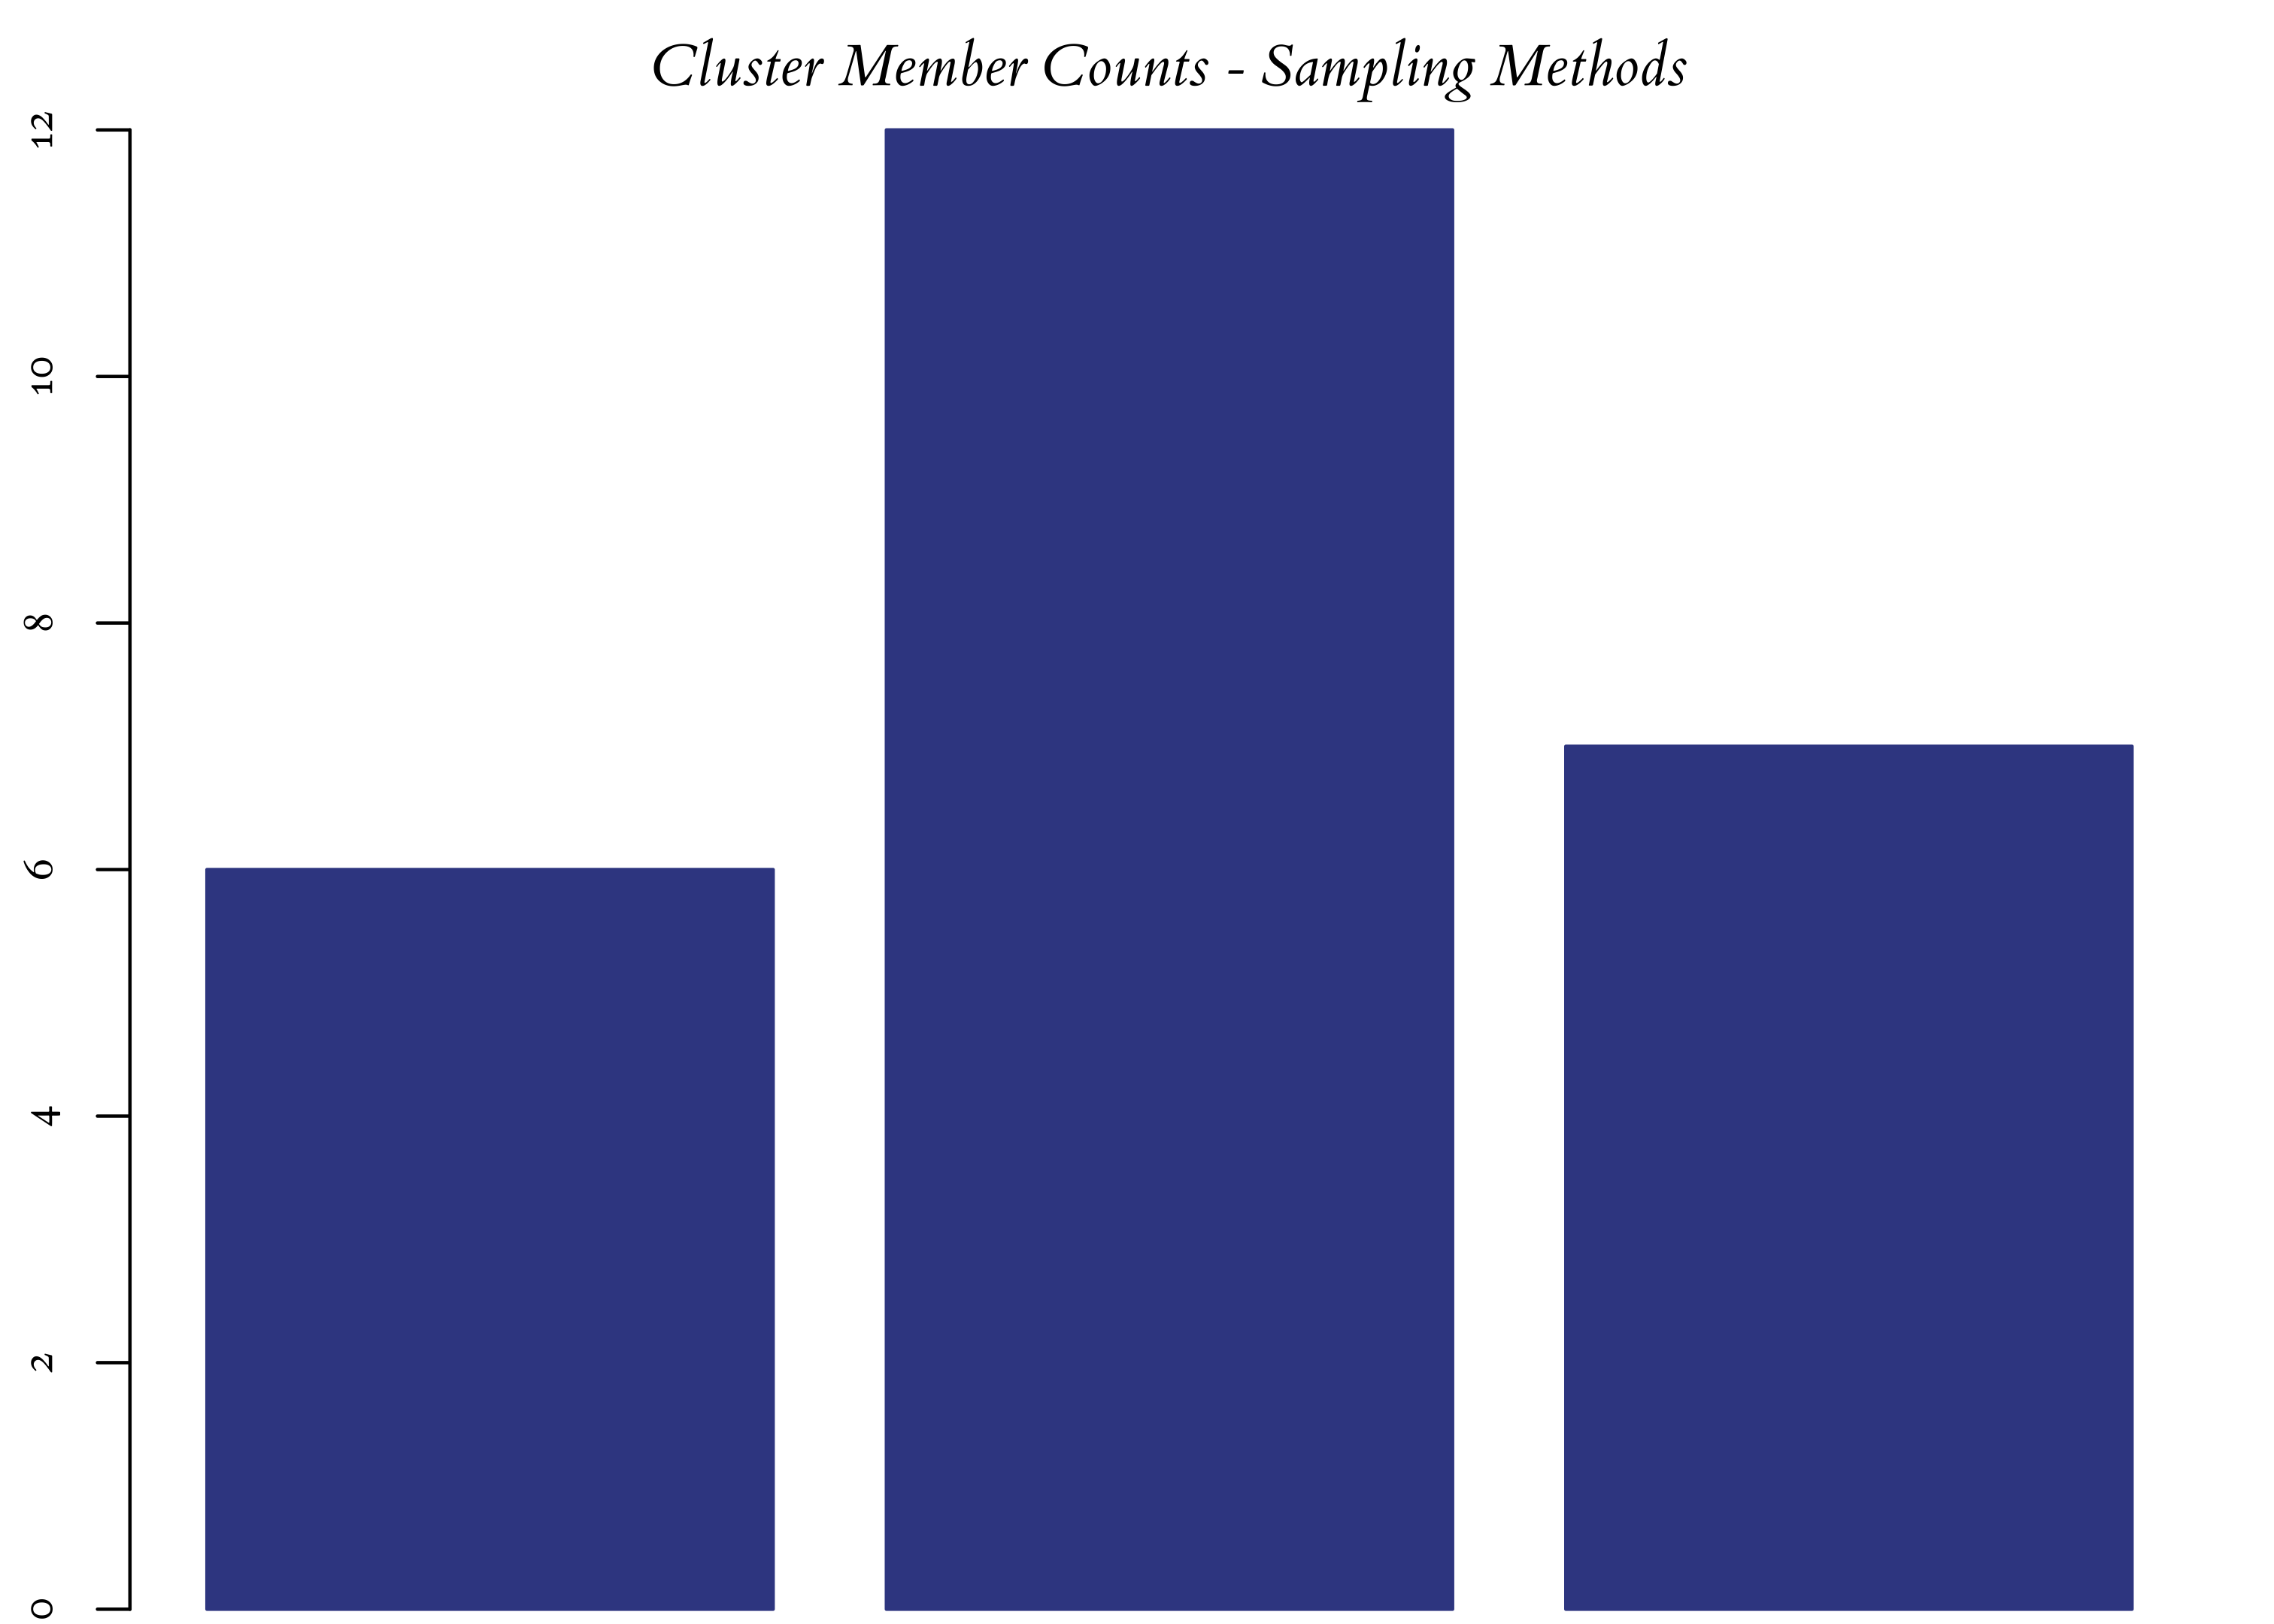
\includegraphics[width=\linewidth]{graphics/rplot-unnamed-chunk-2-2}

\section{IPV-Related Journals}\label{ipv-related-journals}

The following is for determining which IPV-related journals to include
in the formal literature searches conducted for this review.

The data below contain the publication names and corresponding count of
articles from each publication resulting from the inital broad-strokes
database search\footnote{The initial broad-strokes IPV-related
  literature search was conducted using the following command-line
  search:
  ``\texttt{SU(\textquotesingle{}intimate\ partner\ violence\textquotesingle{}\ OR\ \textquotesingle{}domestic\ violence\textquotesingle{}\ OR\ \textquotesingle{}partner\ abuse\textquotesingle{})\ AND\ YR(\$\textgreater{}1965\$)}''}

\Rrule

\begin{Shaded}
\begin{Highlighting}[]
\NormalTok{dat2 <-}\StringTok{ }\KeywordTok{read.csv}\NormalTok{(}\StringTok{"data/ipvJournalsSearch.csv"}\NormalTok{)[}\KeywordTok{c}\NormalTok{(-}\DecValTok{1}\NormalTok{, -}\DecValTok{6}\NormalTok{, -}\DecValTok{7}\NormalTok{), ]}
\NormalTok{## Exclude Theses and Dissertations ##}

\NormalTok{m.cnt <-}\StringTok{ }\KeywordTok{mean}\NormalTok{(dat2[, }\DecValTok{2}\NormalTok{])}
\NormalTok{s.cnt <-}\StringTok{ }\KeywordTok{sd}\NormalTok{(dat2[, }\DecValTok{2}\NormalTok{])}

\NormalTok{dat2.m <-}\StringTok{ }\NormalTok{dat2[dat2[, }\DecValTok{2}\NormalTok{] >=}\StringTok{ }\NormalTok{m.cnt, ]}
\NormalTok{dat2.s <-}\StringTok{ }\NormalTok{dat2[dat2[, }\DecValTok{2}\NormalTok{] >=}\StringTok{ }\NormalTok{s.cnt, ]}
\end{Highlighting}
\end{Shaded}

\begin{longtable}[]{@{}rlr@{}}
\caption{Journals with article counts greater than or equal to the mean
of all journal article counts in the `broad-strokes' database search
results set}\tabularnewline
\toprule
\begin{minipage}[b]{0.11\columnwidth}\raggedleft\strut
~\strut
\end{minipage} & \begin{minipage}[b]{0.56\columnwidth}\raggedright\strut
journal\strut
\end{minipage} & \begin{minipage}[b]{0.09\columnwidth}\raggedleft\strut
count\strut
\end{minipage}\tabularnewline
\midrule
\endfirsthead
\toprule
\begin{minipage}[b]{0.11\columnwidth}\raggedleft\strut
~\strut
\end{minipage} & \begin{minipage}[b]{0.56\columnwidth}\raggedright\strut
journal\strut
\end{minipage} & \begin{minipage}[b]{0.09\columnwidth}\raggedleft\strut
count\strut
\end{minipage}\tabularnewline
\midrule
\endhead
\begin{minipage}[t]{0.11\columnwidth}\raggedleft\strut
\textbf{2}\strut
\end{minipage} & \begin{minipage}[t]{0.56\columnwidth}\raggedright\strut
Journal of Interpersonal Violence\strut
\end{minipage} & \begin{minipage}[t]{0.09\columnwidth}\raggedleft\strut
978\strut
\end{minipage}\tabularnewline
\begin{minipage}[t]{0.11\columnwidth}\raggedleft\strut
\textbf{3}\strut
\end{minipage} & \begin{minipage}[t]{0.56\columnwidth}\raggedright\strut
Journal of Family Violence\strut
\end{minipage} & \begin{minipage}[t]{0.09\columnwidth}\raggedleft\strut
883\strut
\end{minipage}\tabularnewline
\begin{minipage}[t]{0.11\columnwidth}\raggedleft\strut
\textbf{4}\strut
\end{minipage} & \begin{minipage}[t]{0.56\columnwidth}\raggedright\strut
Violence Against Women\strut
\end{minipage} & \begin{minipage}[t]{0.09\columnwidth}\raggedleft\strut
882\strut
\end{minipage}\tabularnewline
\begin{minipage}[t]{0.11\columnwidth}\raggedleft\strut
\textbf{5}\strut
\end{minipage} & \begin{minipage}[t]{0.56\columnwidth}\raggedright\strut
Violence and Victims\strut
\end{minipage} & \begin{minipage}[t]{0.09\columnwidth}\raggedleft\strut
528\strut
\end{minipage}\tabularnewline
\begin{minipage}[t]{0.11\columnwidth}\raggedleft\strut
\textbf{8}\strut
\end{minipage} & \begin{minipage}[t]{0.56\columnwidth}\raggedright\strut
Child Abuse \& Neglect\strut
\end{minipage} & \begin{minipage}[t]{0.09\columnwidth}\raggedleft\strut
246\strut
\end{minipage}\tabularnewline
\begin{minipage}[t]{0.11\columnwidth}\raggedleft\strut
\textbf{9}\strut
\end{minipage} & \begin{minipage}[t]{0.56\columnwidth}\raggedright\strut
Journal of Aggression Maltreatment \& Trauma\strut
\end{minipage} & \begin{minipage}[t]{0.09\columnwidth}\raggedleft\strut
213\strut
\end{minipage}\tabularnewline
\begin{minipage}[t]{0.11\columnwidth}\raggedleft\strut
\textbf{10}\strut
\end{minipage} & \begin{minipage}[t]{0.56\columnwidth}\raggedright\strut
Aggression and Violent Behavior\strut
\end{minipage} & \begin{minipage}[t]{0.09\columnwidth}\raggedleft\strut
176\strut
\end{minipage}\tabularnewline
\begin{minipage}[t]{0.11\columnwidth}\raggedleft\strut
\textbf{11}\strut
\end{minipage} & \begin{minipage}[t]{0.56\columnwidth}\raggedright\strut
Partner Abuse\strut
\end{minipage} & \begin{minipage}[t]{0.09\columnwidth}\raggedleft\strut
159\strut
\end{minipage}\tabularnewline
\begin{minipage}[t]{0.11\columnwidth}\raggedleft\strut
\textbf{12}\strut
\end{minipage} & \begin{minipage}[t]{0.56\columnwidth}\raggedright\strut
Trauma Violence \& Abuse\strut
\end{minipage} & \begin{minipage}[t]{0.09\columnwidth}\raggedleft\strut
132\strut
\end{minipage}\tabularnewline
\begin{minipage}[t]{0.11\columnwidth}\raggedleft\strut
\textbf{13}\strut
\end{minipage} & \begin{minipage}[t]{0.56\columnwidth}\raggedright\strut
Journal of Family Psychology\strut
\end{minipage} & \begin{minipage}[t]{0.09\columnwidth}\raggedleft\strut
114\strut
\end{minipage}\tabularnewline
\begin{minipage}[t]{0.11\columnwidth}\raggedleft\strut
\textbf{14}\strut
\end{minipage} & \begin{minipage}[t]{0.56\columnwidth}\raggedright\strut
Psychology of Violence\strut
\end{minipage} & \begin{minipage}[t]{0.09\columnwidth}\raggedleft\strut
101\strut
\end{minipage}\tabularnewline
\begin{minipage}[t]{0.11\columnwidth}\raggedleft\strut
\textbf{15}\strut
\end{minipage} & \begin{minipage}[t]{0.56\columnwidth}\raggedright\strut
American Journal of Public Health\strut
\end{minipage} & \begin{minipage}[t]{0.09\columnwidth}\raggedleft\strut
100\strut
\end{minipage}\tabularnewline
\begin{minipage}[t]{0.11\columnwidth}\raggedleft\strut
\textbf{16}\strut
\end{minipage} & \begin{minipage}[t]{0.56\columnwidth}\raggedright\strut
Contemporary Psychology\strut
\end{minipage} & \begin{minipage}[t]{0.09\columnwidth}\raggedleft\strut
99\strut
\end{minipage}\tabularnewline
\begin{minipage}[t]{0.11\columnwidth}\raggedleft\strut
\textbf{17}\strut
\end{minipage} & \begin{minipage}[t]{0.56\columnwidth}\raggedright\strut
Social Science \& Medicine\strut
\end{minipage} & \begin{minipage}[t]{0.09\columnwidth}\raggedleft\strut
93\strut
\end{minipage}\tabularnewline
\begin{minipage}[t]{0.11\columnwidth}\raggedleft\strut
\textbf{18}\strut
\end{minipage} & \begin{minipage}[t]{0.56\columnwidth}\raggedright\strut
Issues in Mental Health Nursing\strut
\end{minipage} & \begin{minipage}[t]{0.09\columnwidth}\raggedleft\strut
92\strut
\end{minipage}\tabularnewline
\begin{minipage}[t]{0.11\columnwidth}\raggedleft\strut
\textbf{19}\strut
\end{minipage} & \begin{minipage}[t]{0.56\columnwidth}\raggedright\strut
Journal of Women's Health\strut
\end{minipage} & \begin{minipage}[t]{0.09\columnwidth}\raggedleft\strut
88\strut
\end{minipage}\tabularnewline
\bottomrule
\end{longtable}

\begin{longtable}[]{@{}rlr@{}}
\caption{Journals with article counts greater than or equal one standard
deviation of the distribution for all journal article counts in the
`broad-strokes' database search results set}\tabularnewline
\toprule
\begin{minipage}[b]{0.11\columnwidth}\raggedleft\strut
~\strut
\end{minipage} & \begin{minipage}[b]{0.56\columnwidth}\raggedright\strut
journal\strut
\end{minipage} & \begin{minipage}[b]{0.09\columnwidth}\raggedleft\strut
count\strut
\end{minipage}\tabularnewline
\midrule
\endfirsthead
\toprule
\begin{minipage}[b]{0.11\columnwidth}\raggedleft\strut
~\strut
\end{minipage} & \begin{minipage}[b]{0.56\columnwidth}\raggedright\strut
journal\strut
\end{minipage} & \begin{minipage}[b]{0.09\columnwidth}\raggedleft\strut
count\strut
\end{minipage}\tabularnewline
\midrule
\endhead
\begin{minipage}[t]{0.11\columnwidth}\raggedleft\strut
\textbf{2}\strut
\end{minipage} & \begin{minipage}[t]{0.56\columnwidth}\raggedright\strut
Journal of Interpersonal Violence\strut
\end{minipage} & \begin{minipage}[t]{0.09\columnwidth}\raggedleft\strut
978\strut
\end{minipage}\tabularnewline
\begin{minipage}[t]{0.11\columnwidth}\raggedleft\strut
\textbf{3}\strut
\end{minipage} & \begin{minipage}[t]{0.56\columnwidth}\raggedright\strut
Journal of Family Violence\strut
\end{minipage} & \begin{minipage}[t]{0.09\columnwidth}\raggedleft\strut
883\strut
\end{minipage}\tabularnewline
\begin{minipage}[t]{0.11\columnwidth}\raggedleft\strut
\textbf{4}\strut
\end{minipage} & \begin{minipage}[t]{0.56\columnwidth}\raggedright\strut
Violence Against Women\strut
\end{minipage} & \begin{minipage}[t]{0.09\columnwidth}\raggedleft\strut
882\strut
\end{minipage}\tabularnewline
\begin{minipage}[t]{0.11\columnwidth}\raggedleft\strut
\textbf{5}\strut
\end{minipage} & \begin{minipage}[t]{0.56\columnwidth}\raggedright\strut
Violence and Victims\strut
\end{minipage} & \begin{minipage}[t]{0.09\columnwidth}\raggedleft\strut
528\strut
\end{minipage}\tabularnewline
\begin{minipage}[t]{0.11\columnwidth}\raggedleft\strut
\textbf{8}\strut
\end{minipage} & \begin{minipage}[t]{0.56\columnwidth}\raggedright\strut
Child Abuse \& Neglect\strut
\end{minipage} & \begin{minipage}[t]{0.09\columnwidth}\raggedleft\strut
246\strut
\end{minipage}\tabularnewline
\begin{minipage}[t]{0.11\columnwidth}\raggedleft\strut
\textbf{9}\strut
\end{minipage} & \begin{minipage}[t]{0.56\columnwidth}\raggedright\strut
Journal of Aggression Maltreatment \& Trauma\strut
\end{minipage} & \begin{minipage}[t]{0.09\columnwidth}\raggedleft\strut
213\strut
\end{minipage}\tabularnewline
\begin{minipage}[t]{0.11\columnwidth}\raggedleft\strut
\textbf{10}\strut
\end{minipage} & \begin{minipage}[t]{0.56\columnwidth}\raggedright\strut
Aggression and Violent Behavior\strut
\end{minipage} & \begin{minipage}[t]{0.09\columnwidth}\raggedleft\strut
176\strut
\end{minipage}\tabularnewline
\bottomrule
\end{longtable}



\end{document}
